\section{Тенденции развития позиционных пневмоприводов}\label{sec:ch1/sec2}

Значительный вклад в развитие позиционных пневмоприводов связан с работами И.Б. Филиппова, который в начале 1980-x
годов впервые предложил и теоретически обосновал концепцию пневмопривода с переменной структурой \cite*{филиппов:позиц_след_пневмопривод}.
Разработанная им инновационная схема пневмопривода для промышленных роботов, представленная на рисунке \ref*{fig:phillipov_positioning},
позволила преодолеть фундаментальные ограничения, связанные со сжимаемостью воздуха как рабочей среды.

\begin{figure}[ht]
	\centerfloat
	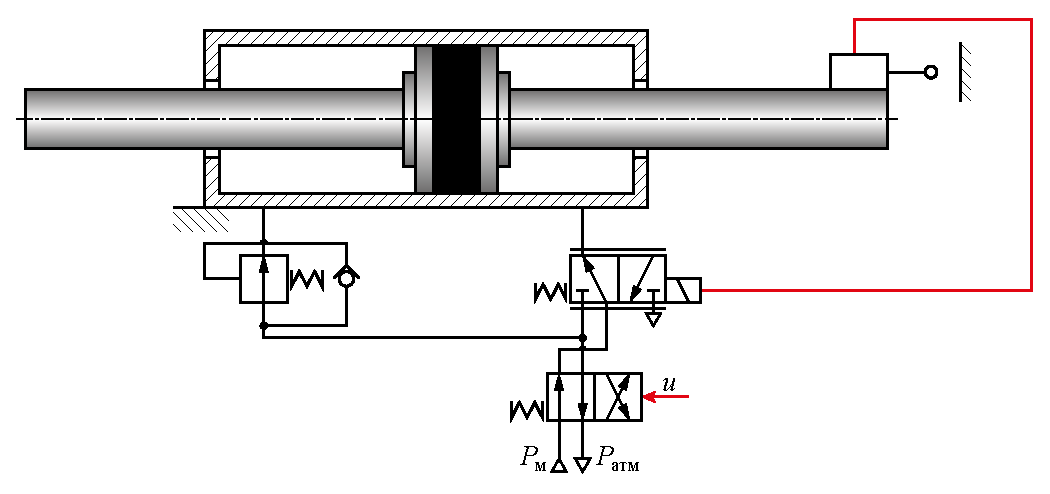
\includegraphics{phillipov_pp.eps}
	\caption{Схема позиционного пневмопривода}\label{fig:phillipov_positioning}
\end{figure}

Принципиальной особенностью предложенной Филипповым системы является комбинирование релейного и следящего режимов
работы: релейный режим используется на участках разгона и установившегося движения, а следящий -- при торможении и
точном позиционировании. Такой подход, реализованный за счет введения
пропорционального распределителя и датчика обратной связи, обеспечивает возможность
позиционирования в произвольной точке хода поршня. При этом параметры привода адаптивно
изменяются в зависимости от текущей координаты позиционирования, что позволяет обеспечить требуемую
точность останова и устойчивость системы \cite*{shortnikov:a}.

% Возрастающие требования к точности позиционирования и быстродействию электропневматических систем определяют
% необходимость учета их специфических особенностей при проектировании. Позиционные пневмоприводы, являясь
% системами с переменной структурой, характеризуются существенной нелинейностью динамических процессов и
% параметрической нестабильностью в процессе работы, что требует разработки специальных подходов к их
% исследованию и эксплуатации.

Работы Филиппова заложили фундаментальные основы создания позиционных пневмоприводов с переменной структурой. Дальнейшее развитие
этого направления осуществлялось в рамках двух основных задач: повышение быстродействия привода и обеспечение
точности позиционирования. При этом особое внимание уделялось проблеме эффективного торможения после участка
разгона, поскольку именно этот этап во многом определяет итоговую точность позиционирования.

В области повышения быстродействия существенный вклад внесли исследования Е.В. Герц.
В работах \cite*{герц:скоростной_привод,герц:групповой_привод} Е.В. Герц исследует проблему повышения быстродействия пневматических
приводов в машиностроении. На основе разработанных математических моделей показано, что типовые промышленные пневмоприводы обладают
недостаточной скоростью рабочих органов (\num{0.5}~--~1 \si{\metre\per\square\second}), что не удовлетворяет требованиям ряда технологических процессов,
где необходима скорость 5~--~20 \si{\metre\per\square\second}.
Для решения данной проблемы предложено использование высокоскоростных пневмоприводов со встроенной полостью-резервуаром. Основной принцип повышения скорости
заключается в обеспечении значительного перепада давлений на рабочем поршне: в рабочей полости поддерживается давление близкое
к магистральному (0,5~--~0,7 \si{\mega\pascal}), а в выхлопной – атмосферное.
Исследования показали существенные преимущества таких пневмоприводов: увеличение рабочего усилия и скорости поршня (до \num{5.3} \si{\metre\per\square\second} на коротких ходах),
повышение энергетической эффективности, возможность точной регулировки выпуска воздуха из резервуара. Однако
их конструкция сложнее типовых и требует больших затрат на подготовку и расход сжатого воздуха.
Несмотря на указанные недостатки, использование высокоскоростных пневмоприводов со встроенным резервуаром признано эффективным
решением для повышения быстродействия в ответственных технологических процессах машиностроения.

В работе \cite*{божкова:повышение_быстродействия} рассматривался выбор
оптимальных параметров управления пневматическим приводом промышленного робота.
Целью было обеспечение высокой скорости работы при сохранении требуемой точности позиционирования.

Авторы Л.В. Божкова и О.А. Дащенко предложили повысить быстродействие путем одновременной работы
динамически независимых узлов привода. Это позволяет избежать последовательной активации пневматических двигателей,
что является типичной практикой для современных промышленных роботов.

Для реализации программного управления без обратной связи, авторы дают ряд рекомендаций по наладке системы.
Это позволяет сократить время переналадки, обеспечить плавность и безударность движения. Таким образом, предложенный
подход направлен на повышение производительности промышленных
роботов с пневматическим приводом без ущерба для точности позиционирования.

В патенте Е.А. Рязанова \cite*{патент:рязанов} предложена конструкция позиционного пневмопривода,
в которой управляющая полость исполнительного пневмоцилиндра сообщена с регулируемым
дозатором в виде плавающего поршня с дросселирующим каналом. Запорный элемент входной
камеры дозатора жестко связан с плавающим поршнем, а выходная камера дозатора постоянно
сообщена с управляющей полостью пневмоцилиндра.

Повышение производительности пневмопривода достигается благодаря созданию управляемого
перепада давления на быстроперемещающемся плавающем поршне дозатора из-за дросселирования
потока через канал, а также за счет упрощения конструкции путем организации жесткой связи запорного элемента
с поршнем и обеспечения быстрой прямой подачи рабочей среды из выходной камеры дозатора в
управляющую полость цилиндра. Это ускоряет процессы подачи и перекрытия рабочей среды, повышая
быстродействие и производительность пневмопривода.

В патенте А.А. Кистиченко \cite*{патент:Кистиченко} представлен подход к повышению
быстродействия пневмопривода за счет совершенствования
систем управления. Предложенная конструкция основана на специальной схеме управления пневмораспределителями
и пневмоклапанами, обеспечивающей быстрый выхлоп рабочей среды из полостей пневмоцилиндра при реверсе движения поршня.

В традиционных пневмоприводах необходимость создания разности давлений в рабочих полостях при реверсировании
приводит к выстою поршня, снижающему быстродействие. Предложенное решение устраняет этот недостаток путем управляемой
отсечки полостей цилиндра от магистрали слива. При подходе поршня к точке реверса система поддерживает такой уровень
давления, который обеспечивает быстрое преодоление сил трения и ускорение в обратном направлении.

Управление осуществляется программным устройством на основе информации о положении поршня и давлениях в полостях. Применение
данной конструкции позволяет повысить быстродействие в 3~--~5 раз по сравнению с традиционными решениями.

Развитие пневмопривода шло по пути повышения ускорения и максимальной скорости движения рабочих органов.
Это достигалось за счет использования более совершенных конструкций, обеспечивающих значительный перепад
давлений на поршне, а также совершенствования систем управления для оптимизации процессов реверсирования
движения поршня. Эти исследования позволяли существенно увеличить скорость и ускорение рабочих органов по
сравнению с типовыми решениями.

Параллельно развивалось направление, связанное с совершенствованием систем позиционирования. Здесь следует отметить работы А.А. Парой,
который является одним из первопроходцев в области исследования задач торможения и позиционирования пневмоприводов промышленных роботов.
В своей работе \cite*{парой:способы_торможения} автор статьи отмечает,
что более 40\%
современных промышленных роботов используют пневматические приводы, что объясняется их высокой надежностью и
низкой стоимостью. Пневмоприводы применяются в качестве основного привода в промышленных роботах с
циклическим управлением и грузоподъемностью до 20~$\div$~30~\si{\kilogram}. Конструктивное решение таких роботов
предполагает использование длинноходовых пневмоцилиндров, которые позволяют реализовать режим
торможения в конце хода с помощью специальных тормозных устройств.

Согласно работе, существует два наиболее распространенных способа обеспечения необходимого
тормозного усилия за счет изменения давления в выхлопной полости пневмопривода. Первый способ заключается в
резком уменьшении площади сечения выхлопного отверстия в определенной точке хода с
последующим поддержанием этой площади постоянной до конца хода. Второй способ предполагает
полное перекрытие площади сечения выхлопного отверстия на первом этапе торможения с последующим
открытием до определенной величины и уменьшением до нуля по определенному закону на втором этапе.
Автор статьи предлагает рассмотреть график, иллюстрирующий эти два режима (рисунок \cref*{fig:парой_режимы_торможения}).

\begin{figure}[h]
	\centerfloat
	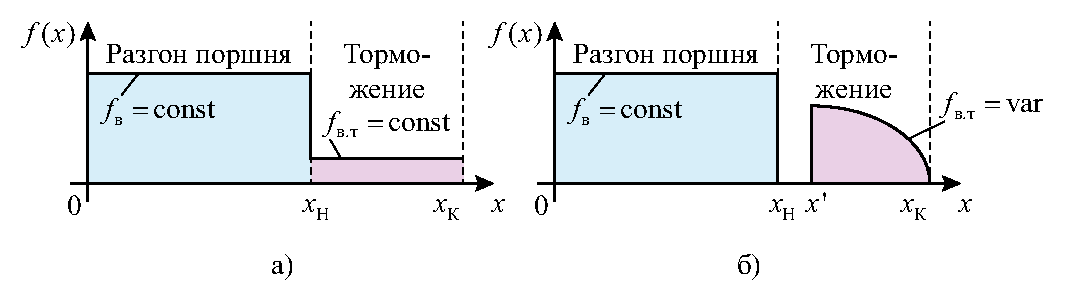
\includegraphics{paroy_brake_mode.eps}
	\caption{Режимы торможения}\label{fig:парой_режимы_торможения}
\end{figure}

Для проектирования тормозных устройств, использующих указанные способы, необходимо определить ряд
параметров, таких как координата начала торможения, площадь сечения выхлопного отверстия,
а также дополнительные координаты и закон изменения площади выхлопа для второго способа.
Автор статьи приводит математические модели, основанные на термодинамических и механических законах,
для расчета этих параметров.

Обобщение накопленного опыта также нашло отражение в разработках Филиппова, где были предложены комплексные решения с использованием
тормозных устройств. В своей монографии, И.Б. Филиппов \cite*{филипов:тормозные_устройства} подробно рассмотрел конструкции и
принципы построения тормозных устройств, применяемых преимущественно для торможения рабочих органов и звеньев машин
с пневмоприводами. Автором была предложена классификация, включающая механические (пружинные, резиновые, эластомерные, инерционные и фрикционные),
пневматические (напорные и вакуумные), гидравлические (дроссельного регулирования), электрические (электромагнитные) и комбинированные тормозные устройства.
Данная класификация представлена на рисунке \cref*{fig:класс_схема_тормозных_устройств}.


\begin{figure}[h]
	\centerfloat
	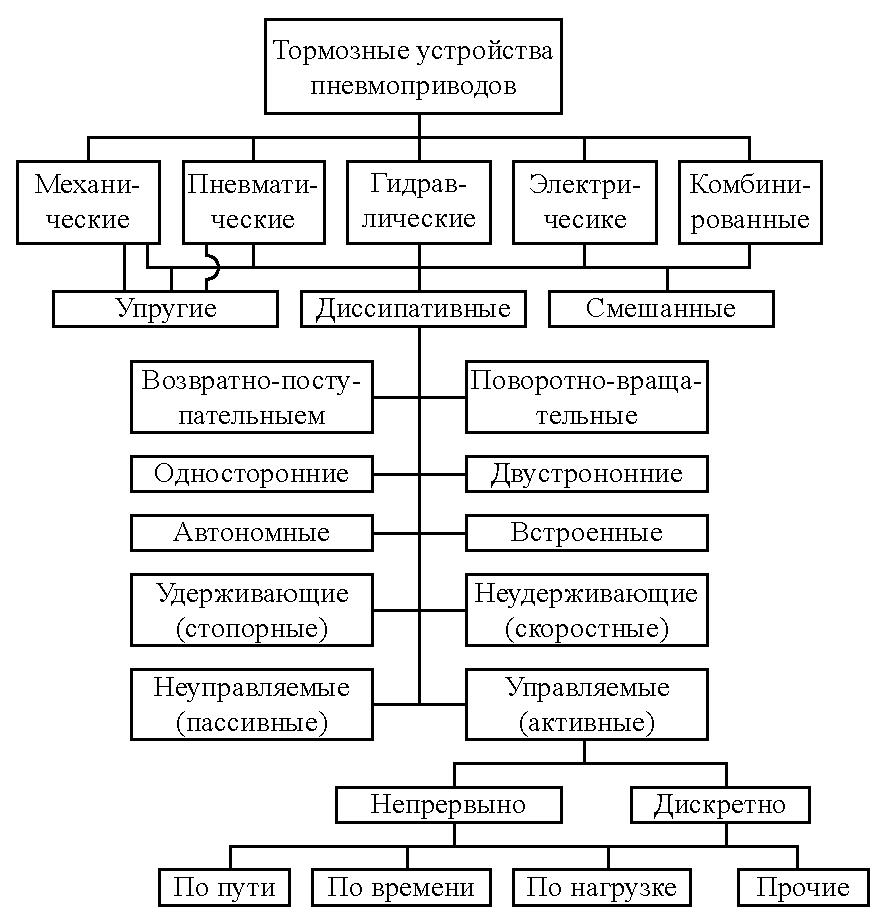
\includegraphics{class_scheme_break.eps}
	\caption{Классификационная схема тормозных устройств}
	\label{fig:класс_схема_тормозных_устройств}
\end{figure}

Выделяются устройства, создающие упругие,
диссипативные или упруго-диссипативные силы сопротивления. Большинство применяемых в настоящее
время тормозных устройств относятся к последнему типу, частично рассеивающих кинетическую энергию и
частично преобразующих ее в потенциальную. Также тормозные устройства могут различаться
по типу движения выходного звена и быть возвратно-поступательными или поворотно-вращательными. Кроме
того они могут быть одностороннего или двустороннего действия.


Особое внимание в работе уделено автономным управляемым тормозным устройствам, которые могут быть унифицированы
и использованы для торможения движущихся масс механизмов с различными типами приводов. Их применение существенно
упрощает задачи компоновки и проектирования, а также эксплуатацию и обслуживание промышленного оборудования.
Автор приводит примеры конструктивного исполнения таких тормозных устройств, в том числе встроенных в пневмоцилиндры
для позиционирования выходного звена.

Помимо этого, в работе изложены основные требования к тормозным устройствам, такие как обеспечение заданного закона
торможения, ограничение ускорений, плавность торможения, высокая надежность и быстродействие, простота и компактность
конструкции, стабильность характеристик и другие. Для оценки эффективности применения тормозных устройств предлагается
использовать показатели, основанные на сравнении кинетической энергии, действующих сил, скоростей, ускорений и других
параметров движения выходного звена до и после их внедрения.

Дальнейшие исследования в области высокоточных быстродействующих пневмоприводов с позиционированием были проведены
В.И. Грищенко и Дао Тхе Аня.

Работа В.И. Грищенко \cite{Grishchenko2010} посвящена разработке позиционного пневмогидравлического привода
с пневмомеханическим контуром управления. Принципиальная особенность привода
заключается в использовании комбинированных пневмогидравлических линий связи и
многофункционального устройства управления на основе вращающегося распределителя.

Конструктивно привод включает силовой пневмоцилиндр, жестко связанный с тормозным
гидроцилиндром, пневмораспределитель, управляющий направлением перемещения исполнительного
механизма, гидрораспределитель, изменяющий структуру гидросистемы, обратный клапан,
регулятор потока и гидроаккумулятор. Ключевым элементом является многофункциональное
устройство управления, содержащее вращающийся распределитель и осевой золотник.

В исходном состоянии поток сжатого воздуха подводится через узел подготовки воздуха к
центральной позиции пневмораспределителя и через распределитель к левому торцу осевого
золотника. При подаче управляющего сигнала поток воздуха поступает в поршневую полость
пневмоцилиндра, обеспечивая ускоренное перемещение исполнительного механизма.

Процесс позиционирования реализуется в три этапа:
\begin{itemize}
	\item разгон выходного звена привода до максимально возможной скорости (\num{1,5}~$\text{м}\cdot\text{с}^{-1}$);
	\item переход на скорость позиционирования путем изменения структуры привода;
	\item установившееся движение на низкой скорости с последующим точным остановом.
\end{itemize}

Автор предложил оригинальное решение по управлению процессом
позиционирования -- использование пневматических линий связи вместо традиционных гидравлических.
Это позволило повысить быстродействие управляющего устройства благодаря более низкой
вязкости воздуха по сравнению с рабочей жидкостью.

Важным практическим результатом работы явилось установление зависимости точности позиционирования
от кинематических параметров привода. Показано, что при увеличении скорости позиционирования
с \num{5} до \num{20}~\si{\milli\metre\per\second} точность остановки исполнительного механизма изменяется от \num{0,01}
до \num{0,05}~\si{\milli\metre}.
При этом поле рассеивания точности не превышает 10~\si{\micro\metre}.

Промышленная апробация подтвердила эффективность предложенного решения. В
координатно-сверлильном полуавтомате достигнута точность позиционирования
по осевой координате \num{0.03}~--~\num{0.04}~\si{\milli\metre} при разбросе выбега \num{0.01}~\si{\milli\metre}.\
В автоматизированном сварочном комплексе обеспечена точность позиционирования
соединений труба-втулка \num{0.1}~--~\num{0.26}~\si{\milli\metre} при различных типоразмерах труб.

В работе Дао Тхе Аня \cite{DaoTheAnh2016} предложен позиционный пневмопривод
повышенного быстродействия и точности.
Автором разработана оригинальная структура привода, включающая силовой пневмоцилиндр, пневмомеханический
контур управления с многопараметрическим датчиком и внешнее тормозное устройство.

В качестве ключевого элемента системы управления используется многопараметрический
пневмомеханический датчик, который преобразует поступательное движение штока пневмоцилиндра
во вращательное движение модулятора через зубчатую передачу. При вращении модулятора формируется
последовательность импульсов давления, несущих информацию о параметрах движения: количество импульсов
пропорционально перемещению, частота -- скорости, амплитуда -- действующей нагрузке. Это обеспечивает
контроль процесса позиционирования в реальном времени.

Особенностью предложенного привода является применение внешнего тормозного устройства с фрикционными
накладками из специальных материалов (Арголон-ТХ, carbenix-4000). Управление тормозом осуществляется
пневматически через электромагнитный распределитель. Такое решение обеспечивает эффективное торможение
и надежную фиксацию механизма в заданной позиции.
Для описания динамики привода автором разработана обобщенная математическая модель в виде системы нелинейных
дифференциальных уравнений. Модель учитывает взаимодействие электромагнитной подсистемы пневмораспределителя,
силовой подсистемы и подсистемы торможения. Проведенные экспериментальные исследования подтвердили адекватность модели.

В результате исследований на специальном стенде установлено, что точность
позиционирования привода составляет \num{40}~--~\num{130}~\si{\micro\metre} при перемещаемых массах
\num{10}~--~\num{17}~кг,
что в \num{2.25} раза превышает показатели серийных пневмоприводов. При этом время
позиционирования сокращено в \num{1.25} раза по сравнению с традиционными решениями.

Разработанное автором программное обеспечение для управления приводом реализовано
на базе программируемого логического контроллера DVP-28SV. Программа формирует
управляющие воздействия на электромагнитные распределители в соответствии с
сигналами датчика и заданным алгоритмом работы. Практическая значимость разработки
подтверждена внедрением в производственную практику ООО <<Камоцци Пневматика>>, где
использование предложенной методики расчета обеспечило сокращение затрат времени и
средств на проектирование приводов на 23\%.





